\section{Problem Definition}

In this section, we define the terminologies and a generic pricing model used in the paper.  At the end we give a formal definition of the problem under consideration.
%Next we define rider request, driver, price models (user and rider profiles), and our optimization goals.

\subsection{Basic Concepts}
The road network is represented as a graph $G(V, E)$, where each node represents intersections, and each edge represents a road segment. 
Each edge $(u,v) \in E$ $(u, v \in V)$ is associated with a weight $c(u,v)$ which is a travel cost (can be time or distance) from $u$ to $v$.
% TODO: define path in road network
The shortest path cost $d(s,t)$ is defined as the minimal cost paths connecting $s$ and $t$. In this paper, time and distance can be converted from one to the other.

\begin{definition} [Ride Request]
\label{def:req}
A ride request r can be represented as $\left\langle s, e, w, f \right\rangle$ consisting of a starting point $s \in V$ and an end point $e \in V$. Each request also specifies $w$ as the maximum time the rider can wait after making a request. In addition, a rider's profile $f: \delta d \rightarrow \left[ 0, 1 \right] $, specifies the relative discount in exchange for an incurred detour of $\delta d$.
%the ridesharing fare she would accept based on the extra detour and the shortest possible trip.
\end{definition}

Upon the acceptance of a request, \fname assigns it to a driver.

\begin{definition} [Driver]
A driver v is a human, driving a vehicle on the road network and is represented as $\left\langle TR, n, g \right\rangle$ where $TR$ is the list of v's assigned ride requests and $n$ is the maximum number of requests v can accept at any point in time. A driver also has a profile $g: d \rightarrow \$ $ which specifies the monetary cost of v driving a distance d while servicing its assigned requests.
\end{definition} 

\begin{definition} [Schedule]
Given a set $TR$ with n requests, a schedule $s= \left\langle x_1, \cdots, x_{2n} \right\rangle$ is an ordered sequence of pickup and delivery points for these request, where for each $r_i \in TR$, $r_i.s$ preceds $r_i.e$ in $s$. 
\end{definition}

A schedule is \textit{valid} for driver \textit{v}, if it satisfies the following conditions:

\begin{itemize}
\item waiting time constraint
\item capacity constraint
\item profit constraint, which is the price constraint based on rider and driver profiles. \moedit{need a more formal definition for this}
\end{itemize}

The driver will follow the sequence of picking up and dropping off riders. The schedule changes over time as riders are picked-up/dropped-off and new requests are added to the schedule. In fact, adding a new request to a schedule, may re-order some of the request that already exist in the schedule.

\begin{definition} [Matching]
Assuming we have a set of Drivers V and a set of Requests R, we call $M \subset V \times R$ a matching if for each $r \in R$ there is at most one $v \in V$ such that $\left( v, r \right) \in M$. We call $\left( v, r \right) \in M$ a \emph{match} and say $r$ has been matched to $v$.
\end{definition}

\noindent In a matching $M$, for every driver $v$, there exists a valid schedule $s_v$, such that $(v, r_i) \in M \implies r_i.s \in s_v \wedge r_i.e \in s_v$ (or simply $r_i \in s_v$). 

\subsection{Pricing Model}

Following the definition of basic concepts in the ride sharing system, we introduce a general price model that can be utilized to compute the corresponding fare of a ride, the payment drivers receive and subsequently, the profit the ride sharing system generates. Before we continue, it is necessary to point out that one of the building blocks of any real-world ride sharing system is a mechanism for computing the shortest path between any two points in the road network. Without loss of generality, we define our pricing model based on a static shortest path computations as opposed to time-dependent. However, the definitions can be easily updated to be compatible with time-dependent networks as well. For example, the fare of a ride is dependent on the distance between the pick-up and the drop-off points in a static network where in a time-dependent network it can be dependent on the travel time between those two points or perhaps both distance and travel time.

Every request $r$ has a default fare based on the shortest distance, $d_r$, from $r.s$ to $r.e$. In other words, we have an arbitrary function $FARE: d \rightarrow \$ $ such that $FARE(d)$ is the default fare of a ride. In a ride sharing system, the actual route between the pick-up and drop-off locations of a ride is not necessary the shortest route between the two points. We show the actual route between the two end points of a ride with $d'_r$ and define the detour of a ride as $\delta d_r = d'_r - d_r$. As explained in \cref{def:req}, each request is associated with a profile. We introduce the concept of a \textit{rider's profile} as a tool for the rider to specify how much discount she expects to receive in return for a certain amount of detour on her trip. A rider's profile can have different formats: linear decay, exponential decay, etc. \cref{fig:rider_profile} shows an example of a rider's profile.

\begin{figure}[!ht]
	\centering
	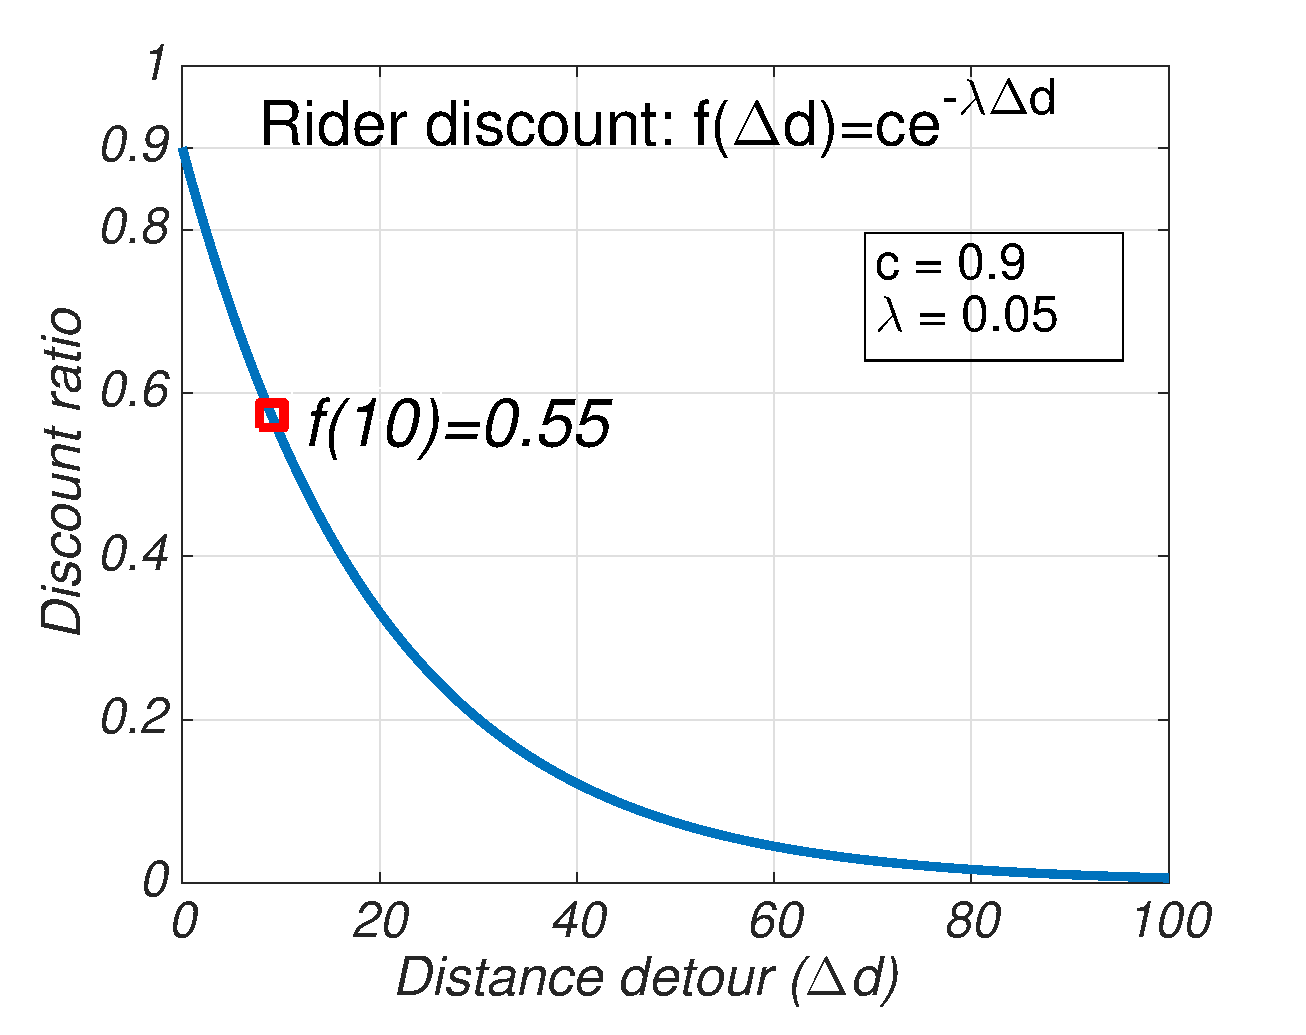
\includegraphics[width = 60mm]{fig/rider.eps}
	\vspace{-0mm}\caption{Rider profile} \vspace{-2mm} \label{fig:rider_profile}
\end{figure}\vspace{-0mm}

Subsequently, for a request $r$ with shortest distance $d_r$, detour $\delta d_r$ and a profile $f_r$, the final fare is:

\begin{equation}
\label{eq:fare}
fare(r) = F(d_r) f_r(\delta d_r)
\end{equation}

Every driver has a unique profile which allows him to specify the cost of his service. Similar to a rider, a driver's profile can be any function. In fact, the function can take any arbitrary input in addition to the distance. For example, it is possible to define the driver's profile as $g: n, d \rightarrow \$$ where $n$ is the number of passengers being serviced by the driver. Without loss of generality, in this paper we assume distance is the only input of the profile. Intuitively, the profile is a monotonically increasing function. For example, the profile in \cref{fig:driver_profile} is one where the driver charges \$1 per mile.

\begin{figure}[!ht]
	\centering
	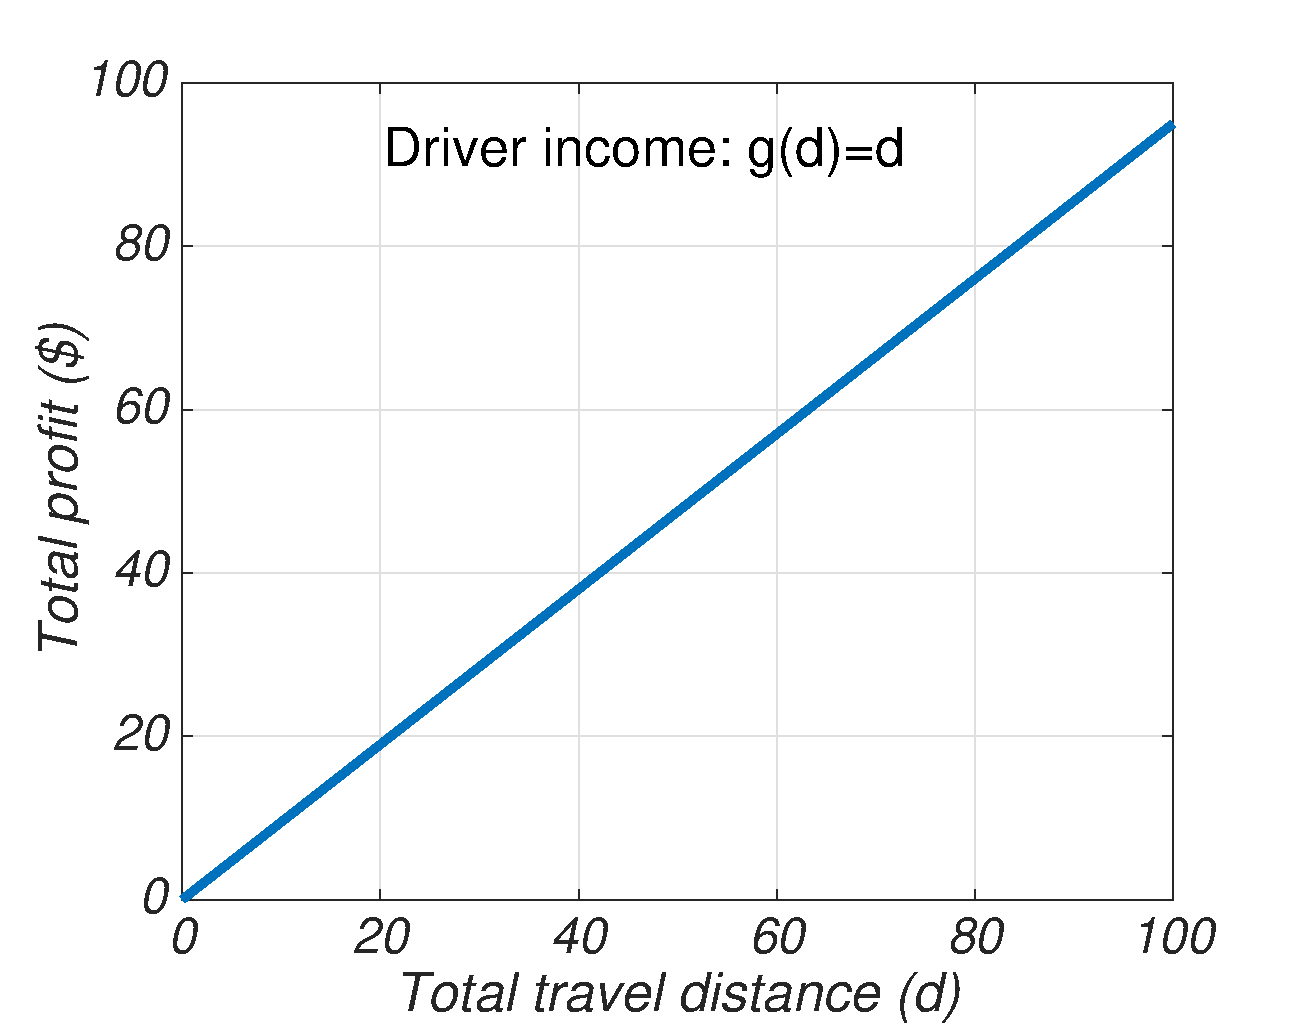
\includegraphics[width = 60mm]{fig/driver.eps}
	\vspace{-0mm}\caption{Driver profile} \vspace{-2mm} \label{fig:driver_profile}
\end{figure}\vspace{-0mm}
 
At any point in time, each driver has a schedule. A driver will be compensated during the time its schedule is not empty. Therefore, for every driver $v$, the cost is:

\begin{equation}
\label{eq:payment}
cost_v = \int_{start_s}^{end_s} I\left( s_v(t) \neq \left\langle \right\rangle\right).g(dist(t))dt
\end{equation}

\noindent Where $I()$ is the indicator function, $s_v(t)$ and $dist(t)$ are the driver's schedule and the distance he travels at time $t$ respectively. In addition, $start_s$ and $end_s$ are the first pick-up time and last drop-off time of $s_v$.

The profit \fname makes from driver $v$ is the difference between the fares collected from all requests serviced by $v$ and the payment $v$ receives for himself. Subsequently, the total profit (revenue) of the system will be the sum of the profits received from all drivers:

\begin{align}
\label{eq:profit} 
profit_v &= \sum_{r_i \in s_v}fare(r_i) - cost_v\\
revenue &= \sum_{v \in V}profit_v
\end{align}

Now that we have defined a generic pricing model, we can define the \textit{Ride-Sharing} problem as follows:

\begin{definition} [Ride-Sharing Problem]
Given a set of ride requests R and a set of drivers V, the goal of the Ride-Sharing problem is to find a matching M between R and V such that the revenue of M is maximized.
\end{definition}

\dingedit{Justify that our objective function is different with minimizing the travel cost.} \moedit{If we have space at the end, we can give a simple contrary example to prove this.}

\subsection{Cost Analysis}

\begin{itemize}
\item Prove the problem is NP-Complete
\item Prove there is no constant $c > 0$ such that an online algorithm is $c-competetive$.
\end{itemize}

%%% TODO: given a rider and the current schedule, calculate the extra profit of inserting a new request.


%Properties of the above definition, can we guarantee the extra profit should be positive?

